\documentclass[11pt]{article}
\usepackage{graphicx}
\usepackage{setspace}
\usepackage{authblk}
\usepackage{url}
\usepackage[inline,shortlabels]{enumitem}
\usepackage[square,numbers]{natbib}
\usepackage{floatrow}
\floatsetup[table]{capposition=top}
\usepackage[nomarkers,nolists]{endfloat}
\usepackage[margin=1in,letterpaper]{geometry}
\usepackage{multirow}
\usepackage[table]{xcolor}
\usepackage[hidelinks]{hyperref}
\usepackage{lineno}
\linenumbers

\bibliographystyle{unsrtnat}

\begin{document}

\title{Adversarial deep neural networks remove nonlinear batch effects from gene-expression data}
\author{Jonathan Bryan Dayton}
\author[1]{Jonathan B. Dayton}
\author[1]{Stephen R. Piccolo}
\affil[1]{Department of Biology, Brigham Young University, Provo, UT 84602 USA}
%[@Please list my contact information. I don't remember how to do this in LaTeX. But please make sure it looks similar to our previous paper.]

\maketitle

\begin{abstract}
	Gene-expression profiling enables researchers to quantify transcription levels in cells, thus providing insights into functional mechanisms of diseases and other biological processes.
	However, because of the high dimensionality of these data and the sensitivity of measuring equipment, expression data often contains unwanted confounding effects that can skew analyses.
	For example, collecting data in multiple runs can cause nontrivial differences in the data known as batch effects.
	In addition, covariates that are not of interest to the study may have strong effects on gene expression.
%	and there may be systemic effects when integrating multiple datasets.
	These confounding effects may be driven by higher-order interactions that are not removable using existing techniques that identify linear patterns.
	We created *Confounded* to remove these effects from expression data.
	[@Please modify the following sentence to better reflect the dual-objective aspect and the fact that it uses neural networks.@]
	Confounded is an adversarial variational autoencoder that removes confounding effects while minimizing the amount of change to the input data.
	We tested the model on artificially constructed data and three gene-expression datasets and compared against other batch-adjustment algorithms.
	Our software is available at \url{https://github.com/jdayton3/Confounded}.
\end{abstract}

\doublespacing
\section{Background} \label{sec:background}

Gene-expression data can be used to advance our understanding of medicine and biology.
For example, gene-expression data have helped to discover conserved genetic modules \citep{stuart_gene-coexpression_2003}, to better understand the mechanisms of cardiovascular disease \citep{henriksen_application_2002}, to more accurately predict clinical outcomes in cancer patients \citep{veer_gene_2002}, and to discover effective drugs for treating specific diseases \citep{sirota_discovery_2011}.
Expression datasets are quite ``wide,'' typically containing tens of thousands of columns representing genes in the human transcriptome.
Because of the sensitive nature of technologies used to generate these data (i.e., expression levels may respond drastically to small environmental changes), expression data often contains unwanted confounding effects that can skew analyses.
Three examples of these include batch effects \label{it:batch}, known covariates, dataset-integration effects.

Batch effects occur when expression data are generated in multiple runs or batches and systemic biases affect the runs. Such biases include different technicians operating the equipment or slight temperature differences in the room.
Batch effects often have a measurable impact on high-throughput expression data \citep{leek_tackling_2010}.
For example, in one study, researchers found that, contrary to prior knowledge, expression values from mice and humans clustered more closely by species than by tissue type \citep{yue_comparative_2014};
however, a later rebuttal showed that when accounting for batch effects, the biological samples clustered more closely by tissue type than by species, as initially expected \citep{gilad_reanalysis_2015}.

Systemic biases can be even more pronounced when driven by known covariates.
For example, Dayton and Piccolo performed a pan-cancer analysis of gene-expression values in The Cancer Genome Atlas, identifying patterns associated with cancer-mutation status\citep{dayton_classifying_2017-1}.
We found that a tumor's tissue of origin exerted a strong effect on gene-expression levels.
This signal was so strong that we could predict a given tumor's tissue of origin with near-perfect accuracy using a machine-learning classifier.
However, we sought to identify patterns that were tissue-agnostic, so tissue of origin represented a confounding effect.

%TODO: Move this to Discussion as a future issue to tackle?
%Finally, data integration is a key goal for gene-expression analyses \citep{lazar_batch_2013}.
%As sample sizes increase, so can statistical significance.
%Although batch effects within a single dataset may be somewhat decreased by careful replication of experimental conditions, this is not possible when integrating different datasets. Methods used for batch correction may be used to correct for dataset-integration effects; however, this problem is 
%however, , .

These biases represent cases where data measurements are affected by hidden variables and must be removed for effective analyses (see \figurename{} \ref{fig:workflow}).

\begin{figure}
	\centering
	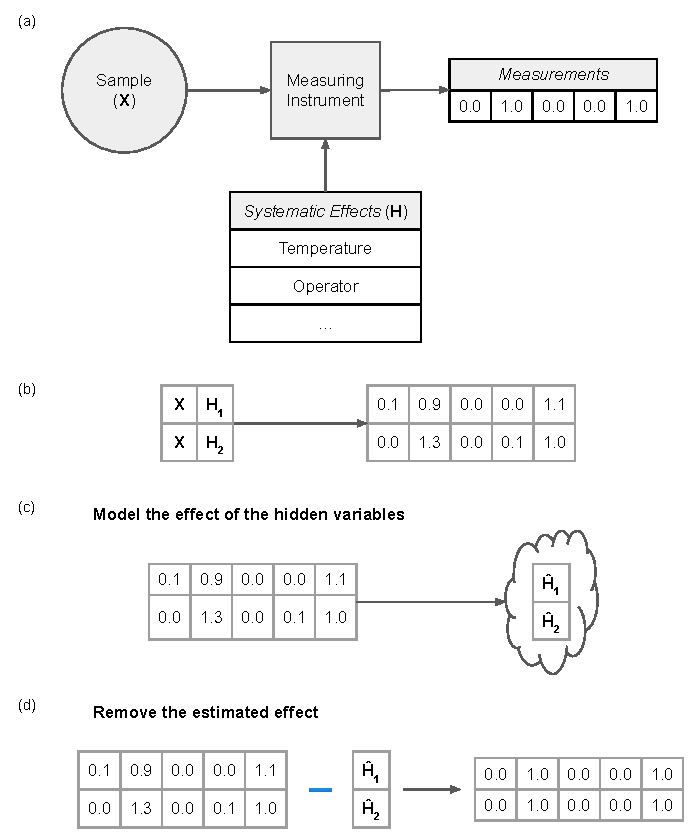
\includegraphics[width=\columnwidth]{figures/final/adjuster_workflow.pdf}
	\caption[Batch adjustment justification and steps]{\textbf{Batch adjustment justification and steps.}
	\begin{enumerate*}[(a)]
		\item When measurements are collected from a sample ($X$), systemic effects ($H$) may affect the measurements.
		\item If data from the same sample $X$ is measured under two different conditions, $H_1$ and $H_2$, we may obtain slightly different measurements.
		\item In order to normalize batches of data relative to one another, we first estimate the effect of the hidden variables based on differences in measurements between batches.
		\item Second, we remove the estimated effects in order to normalize the batches relative to one another.
	\end{enumerate*}
	}
	\label{fig:workflow}
\end{figure}

Several methods exist for characterizing or removing batch effects from gene-expression data.
SVA uses singular value decomposition to model batch effects, which can then be accounted for in statistical analyses\citep{leek_capturing_2007}.
ComBat uses an empirical Bayes approach to estimate batch effect parameters and then uses linear regression to model and remove the effects\citep{johnson_adjusting_2007}.
Both of these techniques use linear methods to model confounding effects and thus may not account for nonlinear effects, such as multi-gene, cascading interactions within signaling pathways.
As machine learning becomes more common in biological research, these nonlinear confounding effects become more troublesome because many machine-learning algorithms can successfully identify such patterns, which may bias the algorithms' outputs.
%For example, advances in neural networks have introduced new ways to account for higher-order, nonlinear relationships in data.
%These networks have proven effective in removing irrelevant, domain-specific signal in credit-rating, online-review, and image-recognition tasks \citep{louizos_variational_2015}.

Artificial neural networks, a category of machine-learning algorithms, are inspired by the way human brains function; input values pass through layers of linear and nonlinear functions; the final output values are measured against specific objectives, and the function layers are adjusted to bring the outputs closer to the objectives; this process is repeated until the outputs are sufficiently close to their targets \citep{schmidhuber_deep_2015}.
Neural networks have been applied broadly to gene-expression data. For example, they have been used to detect cancer and identify critical cancer genes \citep{danaee_deep_2016}, to impute gene-expression levels from the values of a few ``landmark genes'' \citep{chen_gene_2016}, to extract biologically relevant latent spaces in RNA-Seq data \citep{way_extracting_2017}, to reduce the dimensions of single-cell RNA-Seq data \citep{lin_using_2017}, to identify drug-repurposing targets \citep{aliper_deep_2016}, and to generate synthetic biomedical data as a way to preserve patient privacy \citep{beaulieu-jones_privacy-preserving_2017}.

Recent progress has been made in using artificial neural networks to correct batch effects in expression data \cite{shaham_removal_2017,shaham_batch_2018,upadhyay_removal_2019}.
However, these methods are designed for a limited range of scenarios:
1) when the input data contain only two batches,
2) the batches are sufficiently large (batch sizes smaller than 100 failed in our testing), and
3) the batches are balanced.
These requirements rarely hold in applied research; for example, the \textit{bladderbatch} dataset---which is used to test batch-adjustment techniques\cite{leek_bladderbatch_2017,leek_sva_2017}---has 5 batches, 57 samples, and 4 to 19 samples per batch.
Additionally, papers that have described these methods have not evaluated whether nonlinear patterns remain in expression data after batch correction.
To address these limitations, we implemented a deep neural-network architecture that 1) has a batch output layer that expands to fit
the number of batches, 2) works on relatively small batch sizes by sampling with replacement from the training data, and 3) has
no formulas that require batches to be equal sizes.
Furthermore, we tested our method using machine-learning classification algorithms to quantify the extent to which nonlinear batch effects remain after adjustment.

Autoencoders are a type of neural network that encodes input data in a smaller number of dimensions than the original data and then reconstructs the data in the original dimensions\citep{hinton_reducing_2006}.
This technique can be used to reduce noise and thus refine the data representation.[@Make sure this wording is legit. - Are you referencing denoising autoencoders, or are you saying that vanilla autoencoders reduce noise? Either way, we might need a reference. You would know better than I. Please clarify this based on what is relevant to the paper and add a relevant reference.@]
Typically, autoencoders are trained using an objective function that seeks to ensure that the output is as similar as possible to the input \citep{hinton_reducing_2006}.
However, neural networks are adept at finding subtle patterns in data;
thus the objective function may prioritize replication of confounding patterns, such as batch effects, rather than the signals of interest \citep{ganin_domain-adversarial_2015,louizos_causal_2017-2}.
Recently, researchers have experimented with discouraging neural networks from learning such patterns by giving them two competing objective functions:
1) to maximize similarity between in the input and output data and
2) to ignore any patterns associated with known confounding variables \citep{ganin_domain-adversarial_2015,tzeng_deep_2014-2}.
For example, Louizos, et al. used this type of dual-objective function in combination with a variational autoencoder and successfully removed domain-based variability in credit scores, financial savings, and hospital admittance datasets \citet{louizos_variational_2015}.

In this study, we present \textit{Confounded}, an adversarial autoencoder that identifies and removes confounding effects from gene-expression data.
We test the hypothesis that using an adversarial neural network can correct for confounding effects more effectively than alternative tools.
We present a classification-based framework to assess the extent to which confounding effects remain after adjustment, and we apply these techniques to four datasets.

\section{Methods} \label{sec:methods}

An open-source implementation of Confounded is publicly available at \url{https://github.com/jdayton3/Confounded}. Materials for generating this manuscript, including scripts and data, are available at \url{https://github.com/jdayton3/ms-thesis/tree/bioinformatics} and \url{https://osf.io/b76ch/}, respectively.

\subsection{Neural network structure}

We used an adversarial autoencoder network to model and remove confounding effects.
We structured this network in two parts: a variational autoencoder \cite{louizos_variational_2015} to replicate the input (expression) data and a discriminator to detect remaining confounding effects in the autoencoder's output.
By penalizing the autoencoder for the discriminator's success, the autoencoder subnetwork learns over the course of training to output the expression data with confounding effects minimized.
We implemented the neural network in TensorFlow 1.11.0 \cite{abadi_tensorflow_2015} with Python 3.6 \cite{python_software_foundation_python_2019}.
All layers in the network are fully connected, and all activation functions are Rectified Linear Units (ReLUs) \cite{agarap_deep_2018}, except the final layers in the autoencoder and the discriminator, which use the sigmoid function.

\begin{figure}
	\centering
	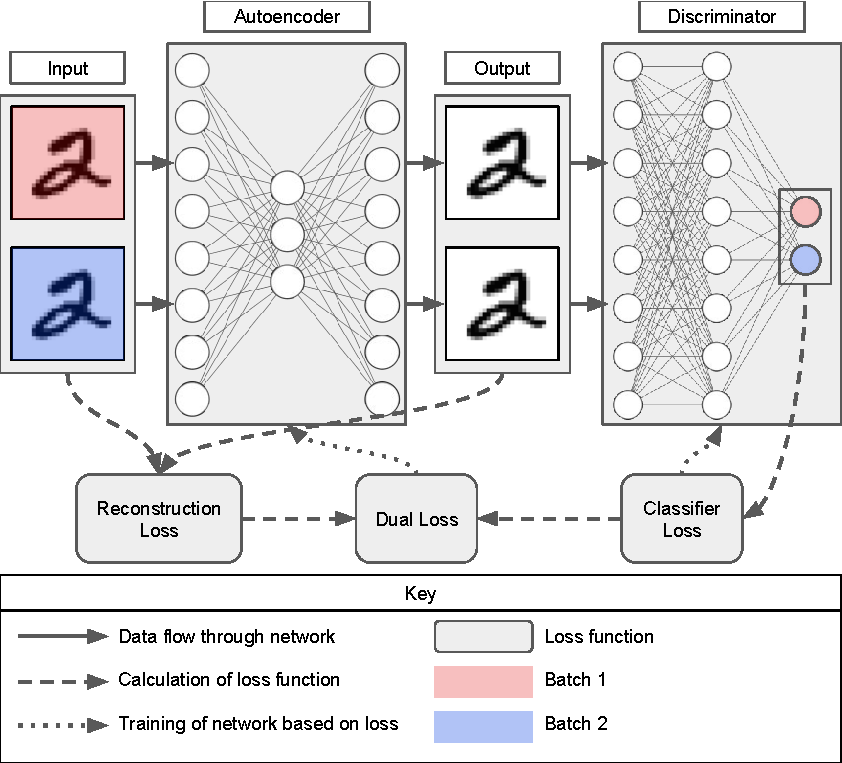
\includegraphics[width=\columnwidth]{figures/final/network.pdf}
	\caption[Network architecture of Confounded]{\textbf{Network architecture of Confounded.}
	Data with batch effects (represented by different colors) are input into an autoencoder.
	The output of the autoencoder is classified by a discriminator network based on batch.
	The autoencoder is then penalized based on the success of the discriminator.
	Over time, the autoencoder learns to output a faithful representation of the data without signal due to batch.}
	\label{fig:network}
\end{figure}

\subsubsection{Autoencoder}

We implemented the variational autoencoder architecture \citep{louizos_variational_2015} described by \citet[Chapter 15]{geron_hands-machine_2017}.
This network has 2 hidden encoding layers and 2 decoding layers, each of size 500.
The code size is 20.
Each hidden layer is activated with the Exponential Linear Unit (ELU) function \citep{clevert_fast_2015} and trained with the Adam optimizer \citep{kingma_adam_2014} on reconstruction loss (sigmoid cross entropy) combined with latent loss (KL divergence \citep{kullback_information_1951}).

\subsubsection{Discriminator}

We trained the discriminator to predict the original batch of the autoencoder's output.
The discriminator subnetwork consists of an input layer; four fully connected hidden layers of sizes 1024, 512, 512, and 128, respectively; and an output layer sized based on the number of batches (i.e. if there are 4 distinct batches in the data, the output layer will be size 4). [@Please provide a little more detail about how the output layer size is calculated - How's this?@].
To combat overfitting and improve training, we also added 50\%-probability dropout \cite{srivastava_dropout_2014} (which prevents overfitting by dropping a random subset of layer inputs in each training iteration) and batch normalization \cite{ioffe_batch_2015} (which helps training by smoothing out the optimization landscape \citep{santurkar_how_2018}) to each layer of the discriminator.
These additions seem to reduce overfitting in the discriminator.

\subsubsection{Loss functions}

We trained the network using three loss functions.
First, we calculated the autoencoder's loss ($L_A$) by summing the reconstruction loss (sigmoid cross entropy between the autoencoder's input and output) and the latent loss (Kullback-Leibler (KL) divergence \cite{kullback_information_1951} of the code layer).
Second, we calculated the discriminator's loss ($L_D$) as sigmoid cross entropy between its output and a one-hot encoding of the samples' batch labels.
Finally, we also trained the autoencoder layers on a combination of the two previous losses,

\begin{equation}
	\label{dual_loss}
	L_{dual} = L_A - \lambda{}(L_D)
\end{equation}

The $\lambda$ value represents a tradeoff parameter for tuning the network's tendency to more faithfully replicate the input or to more completely remove confounding effects.
A higher $\lambda$ value indicates that the network should remove confounding effects more aggressively, whereas a lower value indicates that the network should instead favor faithfully reconstructing the input data.
We did not optimize $L_A$ directly; instead we trained the autoencoder by optimizing $L_{dual}$.

\subsubsection{Training}

In all cases, we trained the network using the Adam Optimizer \citep{kingma_adam_2014} with a training rate of 0.0001 for 10,000 iterations on mini-batches of size 100.
In each iteration, we optimized on both $L_D$ and $L_{dual}$.
When optimizing $L_D$ (i.e. training the discriminator), we froze the autoencoder's weights, and vice versa.
We trained the network on a 2017 Dell XPS 15 9560 with an 8-core Intel i7-7700HQ central processing unit and 16 GB of random access memory.
For each dataset, training took roughly 30 minutes to complete, including time to load the input into memory and to save the output to disk.

\begin{figure}
	\centering
	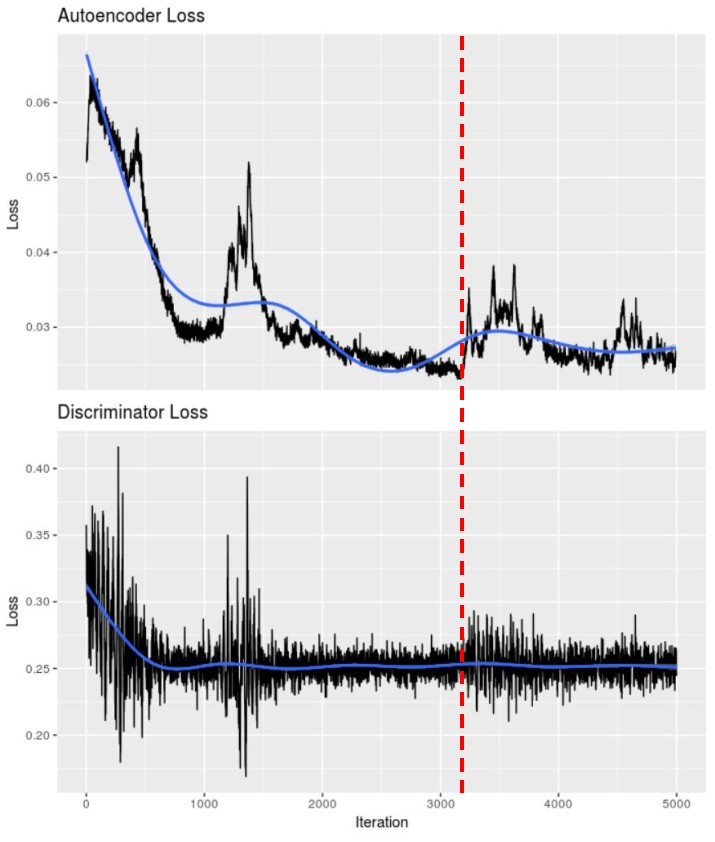
\includegraphics[width=\columnwidth]{figures/final/training_loss.pdf}
	\caption[Autoencoder and discriminator loss]{\textbf{Autoencoder and discriminator loss} over time for one run of Confounded on the MNIST dataset (which we used to validate the network).
	Over the course of training, the autoencoder more faithfully replicates the input data.
	The autoencoder also seems to introduce noise (see the red dashed line near iteration 3100) in response to the discriminator's slight improvements.}
	\label{fig:training_loss}
\end{figure}

\subsection{Comparison to other methods}

We compared Confounded against two other methods that can be used for batch correction. The first was a simple scaling adjuster,
which we implemented in the R programming language (version 3.6.0) \citep{r_core_team_r_2014} using RStudio version 1.2.1194 \citep{rstudio_team_rstudio_2018}.
It adjusts the data by linearly expanding or contracting the values for each variable so that all variables have the same range across the batches.
We also compared against ComBat \citep{johnson_adjusting_2007} using an implementation from the sva package \citep{leek_sva_2017} with some modifications to allow it to work on columns without variance.

We initially intended to test against the SVA \citep{leek_capturing_2007} method but concluded that SVA is more suited for producing surrogate variables for further statistical research rather than removing those variables from the data.
A number of other methods for batch adjustment are available. Some of these use deep neural networks \citep{shaham_removal_2017,shaham_batch_2018,upadhyay_removal_2019}, while others do not\citep{espin-perez_comparison_2018}.
Unfortunately, most of these methods lack a common interface and common assumptions that input datasets must meet.[@This won't be convincing enough to the reviewers. Be more explicit about why we couldn't use these other methods. - Should I just copy the info in the background here (the "limited range of scenarios" part)?@]

\subsection{Datasets}

To test both theoretical and practical differences between Confounded and the alternative methods, we compared them for datasets that varied in size and type of data measured.

\begin{table}
	\centering
	\caption[Dataset information]{
		\textbf{Information} about each dataset used to compare algorithm performance.
	}
	\begin{tabular}{|p{0.18\linewidth}|p{0.14\linewidth}|p{0.1\linewidth}|p{0.15\linewidth}|p{0.23\linewidth}|p{0.16\linewidth}|}
  \hline
  Dataset         & Dimensions   & Number of Batches & Batch Label      & True Class Label       & Data Type        \\
  \hline
  Bladder Batch   & $57\times22,283$  & 5                 & Batch            & Cancer status          & Microarray       \\
  \hline
  GSE37199        & $93\times20,024$  & 2                 & Plate            & Cancer stage           & Microarray       \\
  \hline
  MNIST           & $10,000\times784$ & 2                 & Artificial batch & Digit                  & Grayscale images \\
  \hline
  TCGA Pan-Cancer & $9,366\times325$  & 25                & Cancer Type      & TP53 mutation presence & RNA-Seq \\
  \hline
\end{tabular}

	\label{tab:datasets}
\end{table}

\subsubsection{MNIST}

The MNIST digits dataset \cite{lecun_mnist_nodate} contains images of handwritten digits that are size-normalized and centered.
It contains 60,000 training images and 10,000 test images.
We used MNIST so we could visually assess how well the batch-correction methods preserve true signal (in this case, the shape and digit of each handwritten digit image) after simulated batch adjustment.
We flattened each 28-by-28 image into a 1D vector of size 784 and put each in a CSV file along with the accompanying digit (class) information.
We limited our analysis to the 10,000 test images.
Although convolutional layers are typically used when working with image data, we used fully connected layers to maintain consistency with what would be used on gene-expression data.
However, the autoencoder was still able to represent spatial relationships without explicitly defining them in the model.

\paragraph{Synthetic batch effects}

Because there is no batch information in the MNIST digits dataset, we simulated nonlinear confonding effects.
We applied nonlinear effects by iteratively realizing vectors of normally distributed values, multiplying and adding these vectors to the ``expression'' vectors, and applying nonlinearity to the adjusted vector.
We split the images into two balanced batches (5,000 images for each batch) and included the same number of each digit in each batch.
We applied the same random vectors to each image in a given batch.
Finally, we added random noise to each image to prevent images in a batch from being overly similar to each other.

\subsubsection{Bladderbatch data}

The bladderbatch dataset is a microarray gene-expression dataset from a study of patients with bladder cancer \cite{dyrskjot_gene_2004}.
It is available as an R package \cite{leek_bladderbatch_2017}.
It contains expression values for 57 tissue samples with and without bladder cancer across 5 unbalanced batches.
The dataset has a cancer status (cancerous vs. normal tissue) variable, which we used as the ``true class'' in our validations; it also has a batch variable.
Because bladderbatch is small relative to datasets typically used for deep learning, it helped us to evaluate whether our network overfits on gene-expression datasets of the size often used in applied research.

\subsubsection{GSE37199}

The GSE37199 dataset was profiled using Affymetrix microarrays from patients with advanced castration-resistant prostate cancer \cite{olmos_prognostic_2012}.
We used a curated version of this dataset from \url{http://doi.org/10.17605/OSF.IO/SSK3T}\cite{golightly_curated_2018}.
It contains expression values for 93 tissue samples categorized as either ``Advanced castration resistant'' or ``good prognosis.''
We used these categories for the ``true class'' labels.
This dataset has two types of batch variables---``plate'' and ``centre''---which indicate the microarray plate and research lab that processed the data, respectively.
We adjusted against the ``plate'' variable because it was granular in nature (with counts of $\{43, 50\}$).

\subsubsection{TCGA pan-cancer data}

The Cancer Genome Atlas (TCGA) produced RNA-Sequencing data for tumors across many cancer types \cite{the_cancer_genome_atlas_research_network_cancer_2013}.
In a previous study \cite{dayton_classifying_2017-1}, we classified this dataset based on the presence or absence of mutations in several known cancer genes.
In that study, we observed that cancer type had a strong confounding effect on our analysis, in which sought to identify patterns spanning many cancer types. We adjusted for this effect using ComBat.
However, we found that a strong nonlinear signal could still be identified by the Random Forests algorithm after adjustment.
Here, we used the same version of TCGA dataset (available at \url{https://osf.io/7xjdn/}),
which has expression values for 9,365 samples across 25 cancer types.

\subsection{Statistics and metrics}

\subsubsection{Mean squared error}

Mean squared error (MSE) is a measure of how much two vectors or matrices deviate from one another.
It is commonly used as to quantify loss when the objective (as with autoencoders) is to minimize the difference between input and output values.

\subsubsection{Maximum mean discrepancy} \label{section:mmd}

In a recent paper, \citet{shaham_removal_2017} used neural networks to remove batch effects.
Instead of constraining the autoencoder to remove batch effects based on a discriminator, these researchers trained their network to minimize maximum mean discrepancy (MMD) between batches in an embedded layer of their network.
We calculated MMD using the same formula to determine whether batches appear to come from the same distribution after adjustment.
We used the Gaussian kernel as implemented in \texttt{sklearn.metrics.pairwise.rbf\_kernel} \cite{pedregosa_scikit-learn_2011}.
In cases where there were more than two batches, we averaged all pairwise MMD values to calculate an overall MMD.

\subsubsection{Classification accuracy}

To determine
a) whether batch could still be identified post-adjustment and
b) how well class-related signal was maintained after adjustment,
we used classification algorithms to predict either batch or the ``true class`` labels based on the expression data and used classification accuracy as a metric.
Table \ref{tab:datasets} details which columns were used for these analyses.

We used four classification algorithms from the scikit-learn (version 0.19.1) library \cite{pedregosa_scikit-learn_2011}: Naive Bayes \citep{maron_automatic_1961}, Random Forests \citep{tin_kam_ho_random_1995}, k-Nearest Neighbors \citep{fix_discriminatory_1951}, and SVM \citep{cortes_support-vector_1995} with a radial basis kernel.
In most cases, we used the default hyperparameters, with exceptions of using Random Forests with \texttt{n\_estimators=10} and using SVM with \texttt{kernel="rbf"}.
[@Say something about what hyperparameters we used. Defaults? - How's this?@]

We calculated the average classification accuracy across four-fold cross-validation repeated three times.
We interpreted lower accuracy for batch classification to indicate that batch signal was removed more effectively.
We interpreted higher true-class accuracy to indicate that biologically relevant signal was not lost during the batch-adjustment process.
Therefore, given output data from a ideal batch adjuster, batch classification accuracy would be no better than random chance, and true-class accuracy would be equal to what would be obtained for the unadjusted data.

\section{Results} \label{sec:results}

In this study, we created Confounded, an adversarial, variational, autoencoder neural network, to remove nonlinear confounding effects from gene-expression data that may not be accounted for by linear methods.
We compared Confounded to a scaling method and to ComBat \citep{johnson_adjusting_2007} and used qualitative and quantitative techniques to compare the performance of these methods.
Overall, the scaling method performed consistently worse than the other methods;
ComBat and Confounded each excelled in different scenarios, which we illustrate below.

\subsection{Confounded removes nonlinear confounding effects that other adjusters miss}

[@At least in my mind, we justified using MNIST as a way to visually see how our method performs and to modify it accordingly. However, the Results don't reflect that (in my mind) because the MNIST images are blurry for Confounded, whereas they are clear for the other methods. There is some explanation below about why this might be happening with Confounded. But as an outsider reading this, I would question why we used MNIST at all because our method didn't perform particularly well. It's hard to justify using MNIST anyway because it's so different from gene-expression data. So I think we should remove it from the paper (but it was fine to use it in your thesis). Let me know if you disagree. If not, please remove it. - We talked about maybe keeping it after training for 10k at LR=0.001 and 10k at LR=0.0001. What are your thoughts on this now?@]

[@For simplicity, I think we should only include t-SNE graphs, not PCA. t-SNE accounts for nonlinear patterns, which is the point of our method. - I like including both because it's an evidence that linear visualizations don't cut it when using ML algorithms, but I could go either way on this.@]
[@I also think we should have t-SNE graphs for all three datasets. - Do you think this should be in the main text or just in the supplement?@]
We used principal component analysis (PCA) and t-distributed Stochastic Neighbor Embedding (t-SNE) \citep{maaten_visualizing_2008} plots to visualize the data before and after batch adjustment.
Before any adjustment, batches (microarray plates) in the GSE37199 dataset showed distinct expression patterns for each batch.
After adjustment with each of the three methods, the batches were less distinct (see \figurename{s} \ref{fig:pca} and \ref{fig:tsne}).
In the PCA plot, Confounded appears to maintain a similar distribution to the unadjusted data, indicating that the underlying distribution has been faithfully reproduced by the networks.
The t-SNE plot shows that the data post-adjustment by Confounded and ComBat appear to cluster less tightly by batch than the unadjusted and scale-adjusted data.
This may indicate an effective removal of nonlinear effects in both cases.
%However, previous research has shown that these plots are not completely trustworthy in representing nonlinear effects \cite{dayton_classifying_2017-1}.

\begin{figure}
	\centering
	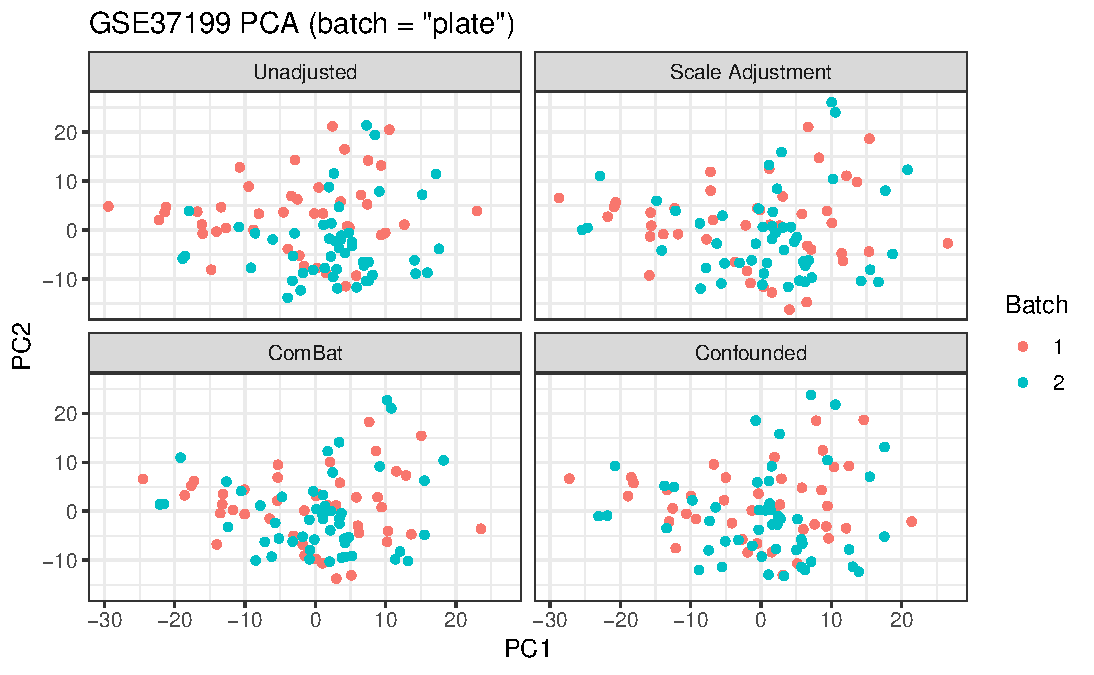
\includegraphics[width=\columnwidth]{figures/final/pca.pdf}
	\caption[Principal components analysis (PCA)]{\textbf{Principal components analysis} (PCA) of the GSE37199 dataset before and after batch adjustment with various adjusters.
	None of the datasets appear to be linearly separable.
	Confounded appears to maintain the same distribution of data overall as the unadjusted data while perhaps aligning the batches' distributions.}
	\label{fig:pca}
\end{figure}
\begin{figure}
	\centering
	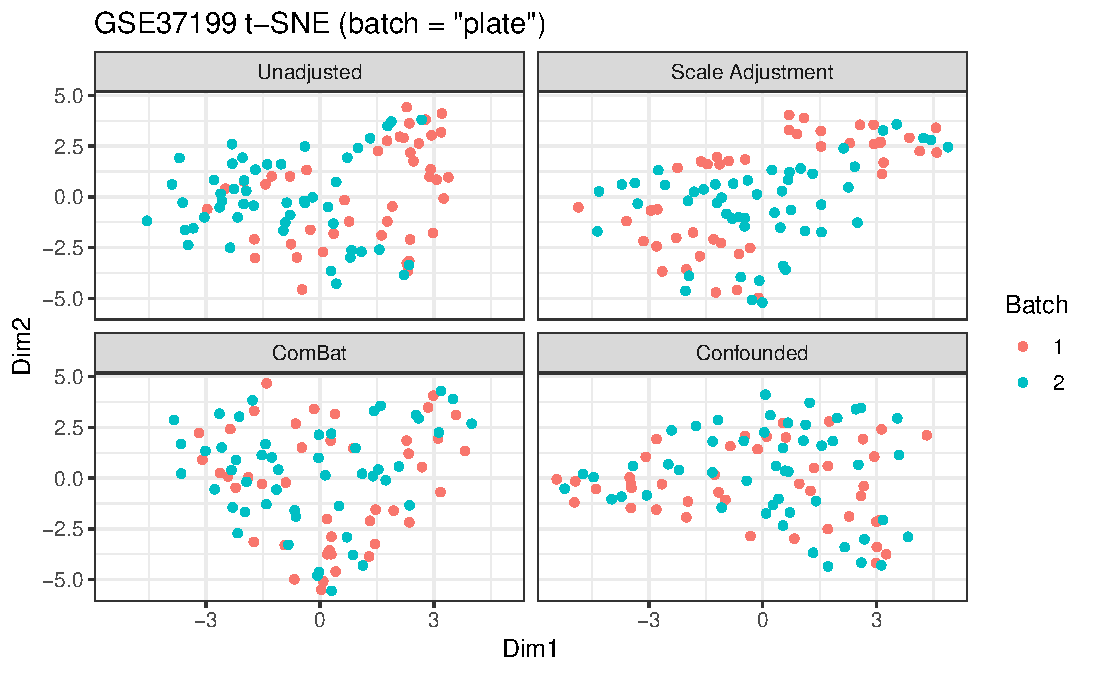
\includegraphics[width=\columnwidth]{figures/final/tsne.pdf}
	\caption[T-distributed Stochastic Neighbor Embedding (t-SNE)]{\textbf{T-distributed Stochastic Neighbor Embedding (t-SNE)} plot for the GSE37199 dataset before and after adjustment with several algorithms.
	The data seem to cluster less by batch for both Confounded and ComBat, indicating that both adjusters may be removing nonlinear effects in this dataset.}
	\label{fig:tsne}
\end{figure}

%%%To compare Confounded against the other batch adjustment methods, we compared PCA and t-SNE plots along with MSE, MMD, and classifier batch prediction accuracy (using various classifiers).
Confounded shows mixed success with the MSE and MMD metrics.
With MSE, Confounded outperformed the scale adjuster in 3 of the 4 datasets but scored drastically worse on the MNIST dataset, with scores listed in Table \ref{tab:mse} (see also \figurename{} \ref{fig:mse}).
With MMD, Confounded outperformed the scale adjuster again in 3 of the 4 datasets and tied the scale adjuster on the TCGA dataset, with scores listed in Table \ref{tab:mmd} (see also \figurename{} \ref{fig:mmd}).
With both metrics, Confounded consistently performed somewhat worse than ComBat.

\begin{figure}
	\centering
	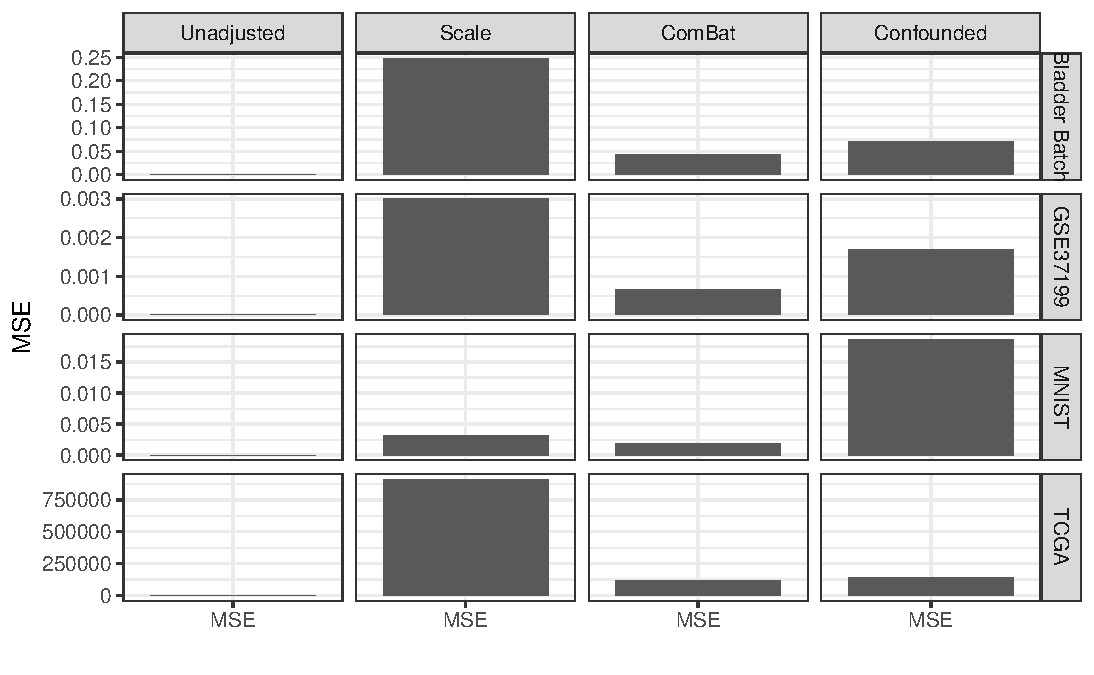
\includegraphics[width=\columnwidth]{figures/final/mse.pdf}
	\caption[Mean squared error (MSE)]{
		\textbf{Mean squared error} (MSE) between the data prior to and after adjustment with various algorithms.
		Lower MSE represents that the adjuster has more faithfully reproduced the input data.
		MSE for unadjusted data will always be 0 because the input data is identical to the output data.
		Confounded usually performs better than the scale adjuster and somewhat worse than ComBat when measuring MSE.
		See also Table \ref{tab:mse}.
	}
	\label{fig:mse}
\end{figure}
\begin{table}
	\centering
\begin{tabular}{l|l|l|l|l}
\hline
Dataset & Unadjusted & Scale & ComBat & Confounded\\
\hline
\rowcolor{gray!6}  Bladder Batch & 0 & 0.247 & 0.0424 & 0.0698\\
\hline
GSE37199 & 0 & 0.003 & 0.00066 & 0.00168\\
\hline
\rowcolor{gray!6}  MNIST & 0 & 0.00312 & 0.00183 & 0.0187\\
\hline
TCGA & 0 & 9.12e+05 & 1.17e+05 & 1.39e+05\\
\hline
\end{tabular}
	\caption[Mean squared error (MSE)]{
		\textbf{Mean squared error (MSE)} of the unadjusted input data compared to the data output by the given adjusters.
		Lower MSE indicates that the output has changed less from the input.
		See also \figurename{} \ref{fig:mse}.
	}
	\label{tab:mse}
\end{table}
\begin{figure}
	\centering
	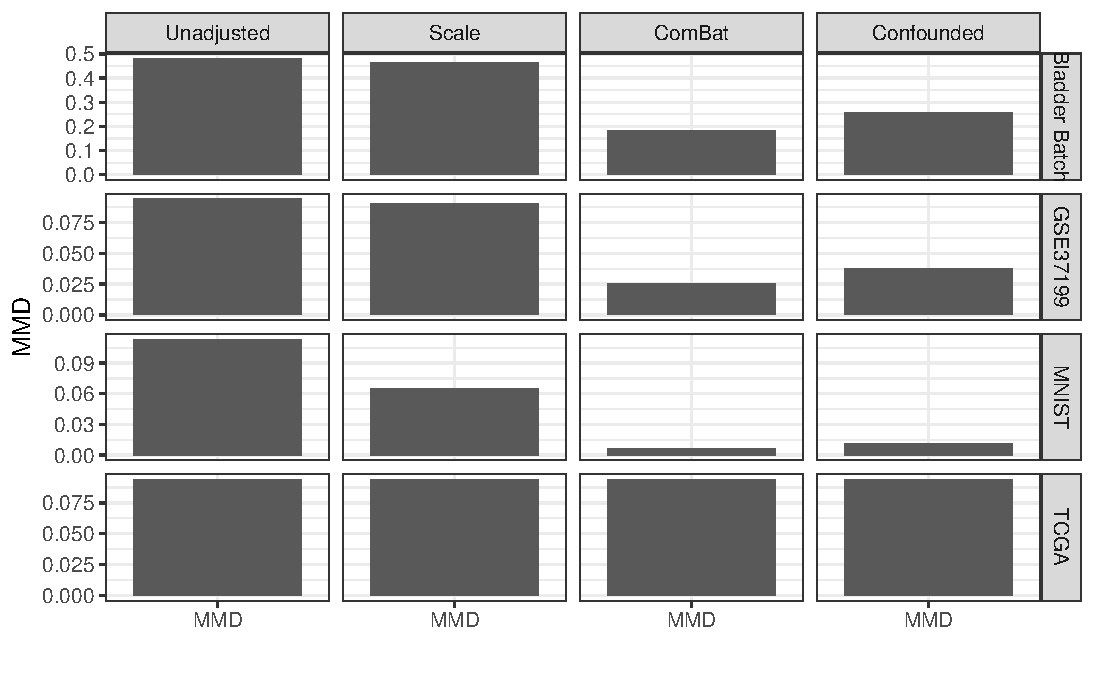
\includegraphics[width=\columnwidth]{figures/final/mmd.pdf}
	\caption[Maximum mean discrepancy (MMD)]{
		\textbf{Maximum mean discrepancy} (MMD) between different batches.
		Lower MMD indicates that the distributions of the different batches are more similar.
		In cases with more than two batches, MMD is computed pairwise between each batch and averaged.
		In each case, Confounded usually performs better than the scale adjuster and somewhat worse than ComBat when measuring MSE.
		See also Table \ref{tab:mmd}.
	}
	\label{fig:mmd}
\end{figure}
\begin{table}
	\centering
	\centering
\begin{tabular}{l|l|l|l|l}
\hline
Dataset & Unadjusted & Scale & ComBat & Confounded\\
\hline
\rowcolor{gray!6}  Bladder Batch & 0.48 & 0.463 & 0.183 & 0.258\\
\hline
GSE37199 & 0.0941 & 0.0906 & 0.0255 & 0.0376\\
\hline
\rowcolor{gray!6}  MNIST & 0.113 & 0.0653 & 0.00665 & 0.0117\\
\hline
TCGA & 0.0942 & 0.0942 & 0.0942 & 0.0942\\
\hline
\end{tabular}
	\caption[Maximum mean discrepancy (MMD)]{
		\textbf{Maximum mean discrepancy} (MMD) comparing the distributions of the batches to each other after a given adjustment.
		Lower MMD indicates that the distributions of the different batches are more similar.
		In cases with more than two batches, MMD is computed pairwise between each batch and averaged.
		See also \figurename{} \ref{fig:mmd}.
	}
	\label{tab:mmd}
\end{table}

We would expect that after batch adjustment by an ideal adjuster, batch would no longer be detectable by any machine learning classifier.
Using the batch classification accuracy metric, Confounded seems to outperform other adjusters on larger datasets, whereas ComBat and Confounded seem to perform about the same on smaller datasets (see \figurename{} \ref{fig:batch}).
With both the bladderbatch and GSE37199 datasets, batch classification accuracy decreases well below baseline after batch adjustment with ComBat for all classifiers we tested (see Table \ref{tab:batch}).
Interestingly, batch accuracy also decreases drastically for the MNIST and TCGA datasets, but only for the Naive Bayes classifier.
This may be due to two factors: both ComBat and Naive Bayes use Bayesian methods, so ComBat may specifically remove the effects that Naive Bayes identifies; and Naive Bayes does not find patterns based on interactions between variables.
Although Naive Bayes is no longer able to identify confounding effects in the data after ComBat-adjustment, Random Forests (which does use interactions between variables) still has a very high accuracy for MNIST and an increased accuracy for TCGA.
In contrast, after adjustment by Confounded, the Random Forests algorithm's accuracy decreases more than with any other adjuster for both the MNIST and TCGA datasets.
This indicates that while ComBat's performance may work at least as well as Confounded for smaller expression datasets, Confounded may work better with larger datasets.

\begin{figure}
	\centering
	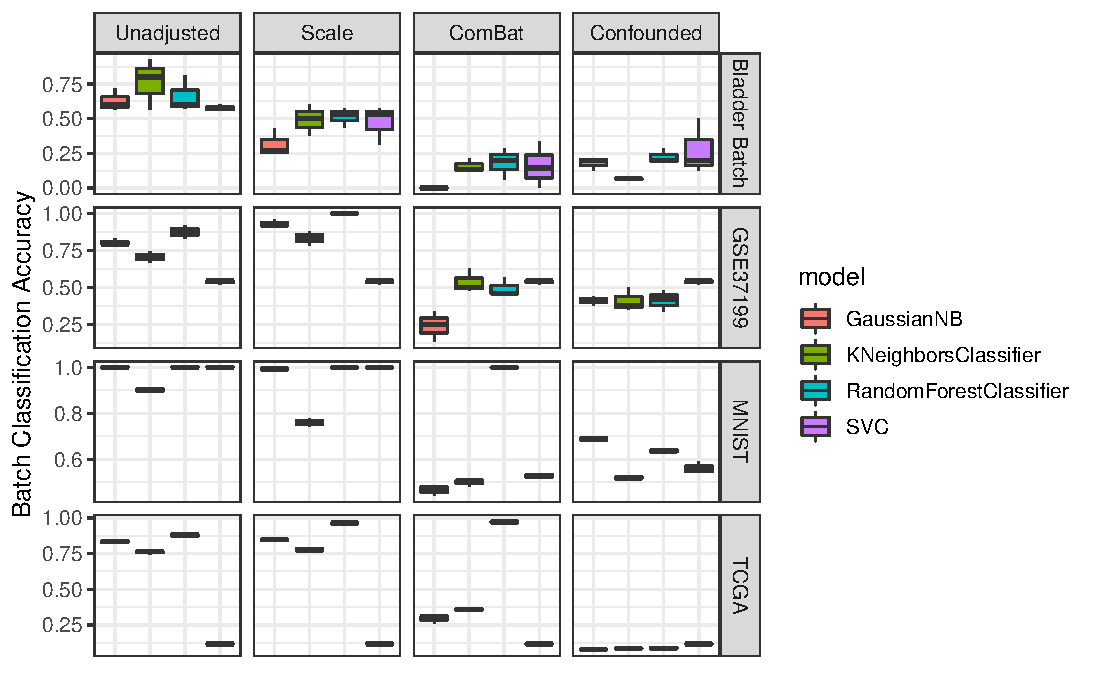
\includegraphics[width=\columnwidth]{figures/final/batch_accuracy.pdf}
	\caption[Batch classification accuracy]{\textbf{Batch classification accuracy} from 4-fold cross-validation repeated 3 times for several classifiers.
	Lower batch accuracy indicates that more batch-related signal has been removed and therefore indicates better performance.
	Confounded's performance is similar to ComBat's for the smaller datasets and is improved for the larger datasets.
	See also Table \ref{tab:batch}.}
	\label{fig:batch}
\end{figure}
\begin{table}
	\centering
	\centering
\begin{tabular}{l|l|r|r|r}
\hline
Dataset & Adjustment & Baseline & GaussianNB & RandomForest\\
\hline
\rowcolor{gray!6}   & unadjusted &  & 0.626 & 0.688\\
\cline{2-2}
\cline{4-5}
 & scale &  & 0.315 & 0.450\\
\cline{2-2}
\cline{4-5}
\rowcolor{gray!6}   & combat &  & 0.000 & 0.114\\
\cline{2-2}
\cline{4-5}
\multirow[t]{-4}{*}{\raggedright\arraybackslash bladderbatch} & confounded & \multirow[t]{-4}{*}{\raggedleft\arraybackslash 0.333} & 0.386 & 0.315\\
\cline{1-5}
\rowcolor{gray!6}   & unadjusted &  & 0.803 & 0.832\\
\cline{2-2}
\cline{4-5}
 & scale &  & 0.930 & 0.928\\
\cline{2-2}
\cline{4-5}
\rowcolor{gray!6}   & combat &  & 0.238 & 0.423\\
\cline{2-2}
\cline{4-5}
 & confounded &  & 0.338 & 0.353\\
\cline{2-2}
\cline{4-5}
\rowcolor{gray!6}  \multirow[t]{-5}{*}{\raggedright\arraybackslash gse37199} & NA & \multirow[t]{-5}{*}{\raggedleft\arraybackslash 0.538} & 0.662 & 0.670\\
\cline{1-5}
 & unadjusted &  & 0.996 & 1.000\\
\cline{2-2}
\cline{4-5}
\rowcolor{gray!6}   & scale &  & 0.998 & 1.000\\
\cline{2-2}
\cline{4-5}
\multirow[t]{-3}{*}{\raggedright\arraybackslash noisy} & combat & \multirow[t]{-3}{*}{\raggedleft\arraybackslash 0.500} & 0.698 & 1.000\\
\cline{1-5}
\rowcolor{gray!6}   & unadjusted &  & 0.832 & 0.879\\
\cline{2-2}
\cline{4-5}
 & scale &  & 0.846 & 0.965\\
\cline{2-2}
\cline{4-5}
\rowcolor{gray!6}  \multirow[t]{-3}{*}{\raggedright\arraybackslash tcga} & combat & \multirow[t]{-3}{*}{\raggedleft\arraybackslash 0.117} & 0.293 & 0.960\\
\hline
\end{tabular}
	\caption[Batch classification accuracy]{
		\textbf{Batch classification accuracy} for several datasets and adjusters.
		The ideal batch adjuster would completely remove all signal due to batch and would therefore \textit{decrease} batch classification accuracy to around the baseline for all classifiers.
		See also \figurename{} \ref{fig:batch}.
	}
	\label{tab:batch}
\end{table}

With the larger datasets in particular, Confounded outperforms the other adjusters.
On the MNIST dataset, Random Forests is able to detect batch with perfect or near-perfect accuracy after adjustment with the scale adjuster and ComBat, but the highest batch classification accuracy after adjustment by Confounded is Naive Bayes, with an accuracy of 68.8\%.
With TCGA, both the scale adjuster and ComBat drastically increase Random Forests' batch classification accuracy from 87.6\% to 96.3\% and 97.1\% respectively, whereas Confounded decreases the accuracy to 8.8\%.

\subsection{Class-related signal is still detectable after adjustment by Confounded}

With the smaller datasets, Confounded seems to keep true class information roughly as well as ComBat, (with Random Forests, Bladderbatch: 74.3 for ComBat\% and 72.1\% for Confounded, GSE37199: 60.4\% for ComBat and 69.0\% for Confounded; see \figurename{} \ref{fig:true_class} and Table \ref{tab:true_class}).
For the Bladderbatch dataset, true class accuracy is much lower after adjusting with any algorithm, indicating that cancer status and batch may not be independent.

With the larger datasets, Confounded's true class accuracy consistently decreases below the accuracy of other adjusters.
A look at the MNIST digits before and after adjustment (see \figurename{} \ref{fig:mnist}) shows that Confounded's output is often blurry, as is common with the output of variational autoencoders \cite{hou_deep_2016}.
With MNIST, Confounded's accuracy with Random Forests is still much higher than baseline (84.8\% vs. 11.4\%), but with TCGA, the accuracy decreases below baseline (66.5\% vs. 69.8\%) while the other adjusters' accuracies remain above baseline.
However, the particular set of parameters that we used in Confounded are likely not optimal for every dataset.
Additional tuning may improve the performance metrics.

\begin{figure}
	\centering
	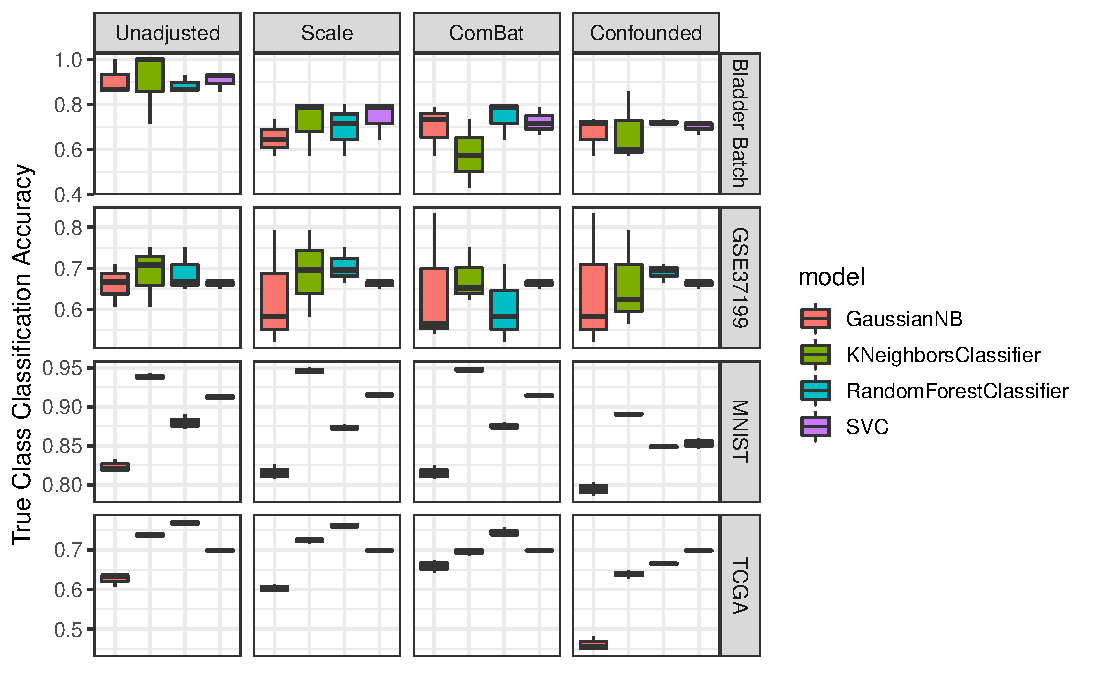
\includegraphics[width=\columnwidth]{figures/final/true_class_accuracy.pdf}
	\caption[True class classification accuracy]{\textbf{True class classification accuracy} for several datasets and adjusters with 4-fold cross-validation repeated 3 times. A higher accuracy after adjustment is desired because it represents that the adjuster has not destroyed the true class signal.
	See also Table \ref{tab:true_class}.}
	\label{fig:true_class}
\end{figure}
\begin{table}
	\centering
	\centering\rowcolors{2}{gray!6}{white}

\begin{tabular}{l|l|r|r|r|r|r}
\hiderowcolors
\hline
Dataset & Adjustment & Baseline & GaussianNB & KNeighbors & RandomForest & SVC\\
\hline
\showrowcolors
 & Unadjusted &  & 0.9079365 & 0.9047619 & 0.8841270 & 0.9063492\\
\cline{2-2}
\cline{4-7}
 & Scale &  & 0.6492063 & 0.7190476 & 0.6952381 & 0.7428571\\
\cline{2-2}
\cline{4-7}
 & ComBat &  & 0.6968254 & 0.5777778 & 0.7428571 & 0.7222222\\
\cline{2-2}
\cline{4-7}
\multirow[t]{-4}{*}{\raggedright\arraybackslash Bladder Batch} & Confounded & \multirow[t]{-4}{*}{\raggedleft\arraybackslash 0.7017544} & 0.6730159 & 0.6761905 & 0.7206349 & 0.6984127\\
\cline{1-7}
 & Unadjusted &  & 0.6612319 & 0.6890097 & 0.6896135 & 0.6618357\\
\cline{2-2}
\cline{4-7}
 & Scale &  & 0.6322464 & 0.6902174 & 0.7041063 & 0.6618357\\
\cline{2-2}
\cline{4-7}
 & ComBat &  & 0.6467391 & 0.6757246 & 0.6044686 & 0.6618357\\
\cline{2-2}
\cline{4-7}
\multirow[t]{-4}{*}{\raggedright\arraybackslash GSE37199} & Confounded & \multirow[t]{-4}{*}{\raggedleft\arraybackslash 0.6666667} & 0.6461353 & 0.6606280 & 0.6902174 & 0.6618357\\
\cline{1-7}
 & Unadjusted &  & 0.8236658 & 0.9388265 & 0.8801867 & 0.9128345\\
\cline{2-2}
\cline{4-7}
 & Scale &  & 0.8160683 & 0.9462902 & 0.8743188 & 0.9153669\\
\cline{2-2}
\cline{4-7}
 & ComBat &  & 0.8152686 & 0.9478891 & 0.8755154 & 0.9140346\\
\cline{2-2}
\cline{4-7}
\multirow[t]{-4}{*}{\raggedright\arraybackslash MNIST} & Confounded & \multirow[t]{-4}{*}{\raggedleft\arraybackslash 0.1135000} & 0.7944837 & 0.8907100 & 0.8484595 & 0.8528601\\
\cline{1-7}
 & Unadjusted &  & 0.6251933 & 0.7380770 & 0.7675432 & 0.6979360\\
\cline{2-2}
\cline{4-7}
 & Scale &  & 0.6028491 & 0.7232736 & 0.7602833 & 0.6979360\\
\cline{2-2}
\cline{4-7}
 & ComBat &  & 0.6590746 & 0.6953731 & 0.7444855 & 0.6979360\\
\cline{2-2}
\cline{4-7}
\multirow[t]{-4}{*}{\raggedright\arraybackslash TCGA} & Confounded & \multirow[t]{-4}{*}{\raggedleft\arraybackslash 0.6979500} & 0.4612043 & 0.6387186 & 0.6651957 & 0.6979360\\
\hline
\end{tabular}
\rowcolors{2}{white}{white}
	\caption[True class classification accuracy]{
		\textbf{True class classification accuracy} for several datasets and adjusters.
		After adjustment by the ideal batch adjuster, all true class signal should be preserved, and all classifiers should therefore have the same accuracy in predicting true class before and after adjustment.
		See also \figurename{} \ref{fig:true_class}.
	}
	\label{tab:true_class}
\end{table}

\begin{figure}
	\centering
	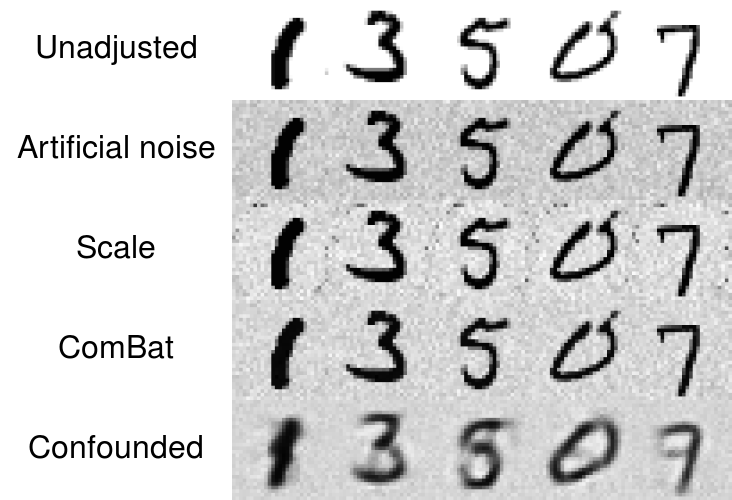
\includegraphics[width=\columnwidth]{figures/final/mnist.png}
	\caption[MNIST handwritten digits]{\textbf{MNIST handwritten digits}
	\begin{enumerate*}[(a)]
		\item before any adjustment,
		\item with artificial noise added,
		\item adjusted for noise by the scale adjuster,
		\item adjusted for noise by ComBat, and
		\item adjusted for noise by Confounded.
	\end{enumerate*}
	Although Confounded seems to remove more noise from the background, it struggles in some cases to accurately replicate the input data.}
	\label{fig:mnist}
\end{figure}

\section{Discussion} \label{sec:discussion}

\textbf{Why should I use a neural network for batch adjustment?}
The process of measuring data typically leaves confounding effects, especially when the data or measurement process involves living things.
Imagine an experiment where two researchers measure the length of caterpillars.
If one researcher is left-eye dominant and the other is right-eye dominant, they may each see lengths as being a millimeter different.
If both researchers use the same wooden ruler at different relative humidities, the measurements may come out differently due to the wood swelling or due to the caterpillars reactions to humidity.
These same types of problems exist when measuring expression levels, but to more of an extreme---in addition to the target values and measuring equipment changing slightly due to systemic factors, the target values also change in response to each other.
Each of the 20,000 transcript levels may influence or be influenced by other transcript levels.
These cascading network-like effects are extremely likely to have nonlinear components, and our research shows that these nonlinear effects do indeed exist in gene expression data, thus rendering linear batch correction methods insufficient.
Therefore, some form of nonlinear adjustment must be used in order to correct for real-world confounding effects.
Rather than individually model each of infinitely many possible nonlinear interactions to see which represent confounders, we can use a neural network to both approximate and remove the confounders, since neural networks are proven to be universal function approximators \citep{csaji_approximation_2001}.

\textbf{How can I tell how well batch adjustment worked?}
Although the metrics and figures that have been used in the past to validate batch adjustment (such as PCA, MSE, and MMD) represent how well linear effects have been removed, they cannot completely display whether two batches are distinguishable from one another.
Machine learning algorithms are designed specifically to tease out patterns in data that may distinguish one group from another.
We suggest to users of batch correction software that they use machine learning classification accuracy before and after correction in order to determine the degree of batch removal.
We also suggest to researchers in the field of batch correction that classification accuracy be used as a metric in validating their software.
Specifically, the Random Forests algorithm \citep{tin_kam_ho_random_1995} seems to work very well and runs relatively quickly on gene expression data.

\textbf{Which batch adjuster should I use?}
In our testing, ComBat did very well with small ($n < 100$) datasets, even with removing any identifiable nonlinear effects.
However, Confounded outperformed ComBat on the larger datasets according to the batch classification accuracy metric.
In addition to dataset size, researchers selecting a batch adjustment algorithm should consider how important it is for them to accurately replicate their input data.
Such researchers can adjust Confounded's $\lambda$ parameter in order to balance the tradeoff of removing batch and matching the inputs.

\textbf{What limitations does Confounded have?}
\begin{enumerate*}[(a)]
	\item Confounded uses a variational autoencoder, which are known for often outputting a blurry version of the input data (as can be seen in \figurename{} \ref{fig:mnist}).
	However, recent work has identified modifications that may be made to the basic VAE structure to make output images sharper and more realistic \citep{hou_deep_2016}.
	Similar research with variational autoencoders and gene expression data may yield improved reconstruction losses and decrease the blurring effect.
	\item Confounded takes a long time to run in comparison with ComBat and other linear adjusters.
	Although we acknowledge this as a downfall of many types of machine learning and of neural network in particular, we believe that 30-60 minutes is a reasonable amount of time for a step that will be run only once per pipeline and that can greatly improve data quality.
	\item It can be difficult to identify the optimal network structure and parameter set for a neural network.
	Though this is the case for many applications of neural networks, we feel that Confounded's default structure worked well in our testing and that it will suffice for most batch correction applications.
	\item Neural networks usually perform better when given large amounts of data, and traditional batch datasets typically have very few samples.
	We did find that ComBat may outperform Confounded on many smaller, more traditional datasets, but that Confounded performs better on larger datasets.
	However, Confounded did perform reasonably well with the smaller datasets and appeared to avoid overfitting.
	In cases where ComBat is unable to completely remove confounding effects in a small dataset, Confounded may be a viable replacement method.
\end{enumerate*}

\textbf{What else might Confounded be used for?}
At its root, batch correction is a data integration problem:
data from multiple batches must have batch-specific confounding effects removed in order to be treated as one dataset.
Confounded shows promise in removing traditional batch effects from microarray expression data in the Bladderbatch and GSE37199 datasets.
It also effectively decreased artificial batch effects in image data and cancer-type-specific confounding effects in RNA-Seq data.
Confounded may be effective in other data integration problems, such as combining microarray with RNA-Seq datasets, or merging several large datasets measured under different conditions.

Confounded, and adversarial autoencoders in general, show promise as a valuable way to remove confounding biases from expression datasets.
Such methods will enable researchers access to larger datasets, therefore increasing the scope of analyses and furthering science as a whole.

\newpage
\phantomsection
\addcontentsline{toc}{section}{References}
\bibliography{references}

\end{document}
